\chapter{Predizione della struttura di proteine (PSP)}

Il protein folding problem ha sia guidato che tratto beneficio dagli avanzamenti nei metodi sperimentali e computazionali\supercite{dill2008protein}. Uno dei maggiori obiettivi della biologia computazionale è proprio il PSP (Protein Structure Prediction), ovvero la predizione della struttura nativa tridimensionale di una proteina a partire dalla sua sequenza amminoacidica. Il PSP è il problema opposto al \textit{protein design} (la progettazione di nuove sequenze proteiche che abbiano delle specifiche attività).

\par Grazie al CASP, alla crescita del PDB e ai metodi per omologia e di allineamento di sequenze i metodi computazionali hanno registrato notevoli progressi, come dimostra il livello raggiunto da AlphaFold. 

\par La predizione della struttura di proteine è uno strumento fondamentale in medicina per la comprensione delle malattie da misfolding, nell'industria farmaceutica per risparmiare anni di laboriosi e costosi esperimenti correntemente richiesti per lo sviluppo di un singolo farmaco (\textit{drug design}), in biotecnologia per il design di nuovi enzimi e in generale per acquisire maggior conoscenza sul protein folding in tutti i suoi lati.

\par La predizione della struttura è importante per un semplice motivo: i biochimici conoscono oggi la sequenza amminoacidica per più di 225 milioni di proteine\supercite{proteienDBentries} (UniProt, con circa 4.5-5 milioni aggiunte ogni mese) ma sono state determinate solamente circa 160.000 strutture tridimensionali di proteine\supercite{proteienDBentries} (PDB\footnote{Al 3 Febbraio 2022 sono presenti 162.913 strutture di proteine nella versione dell'RCSB. Nel PDB ci sono anche strutture di altre macromolecole (complessi di acidi proteici-nucleici, DNA e RNA) per un totale, incluse le proteine, di 186670\supercite{pdbStats}. Nel wwPDB (database globale) vi sono in totale 197961 strutture di macromolecole\supercite{wwpdbStats}.}, con poco più di 10.000 strutture aggiunte ogni anno). 

\begin{figure}[!htb]
	\centering
	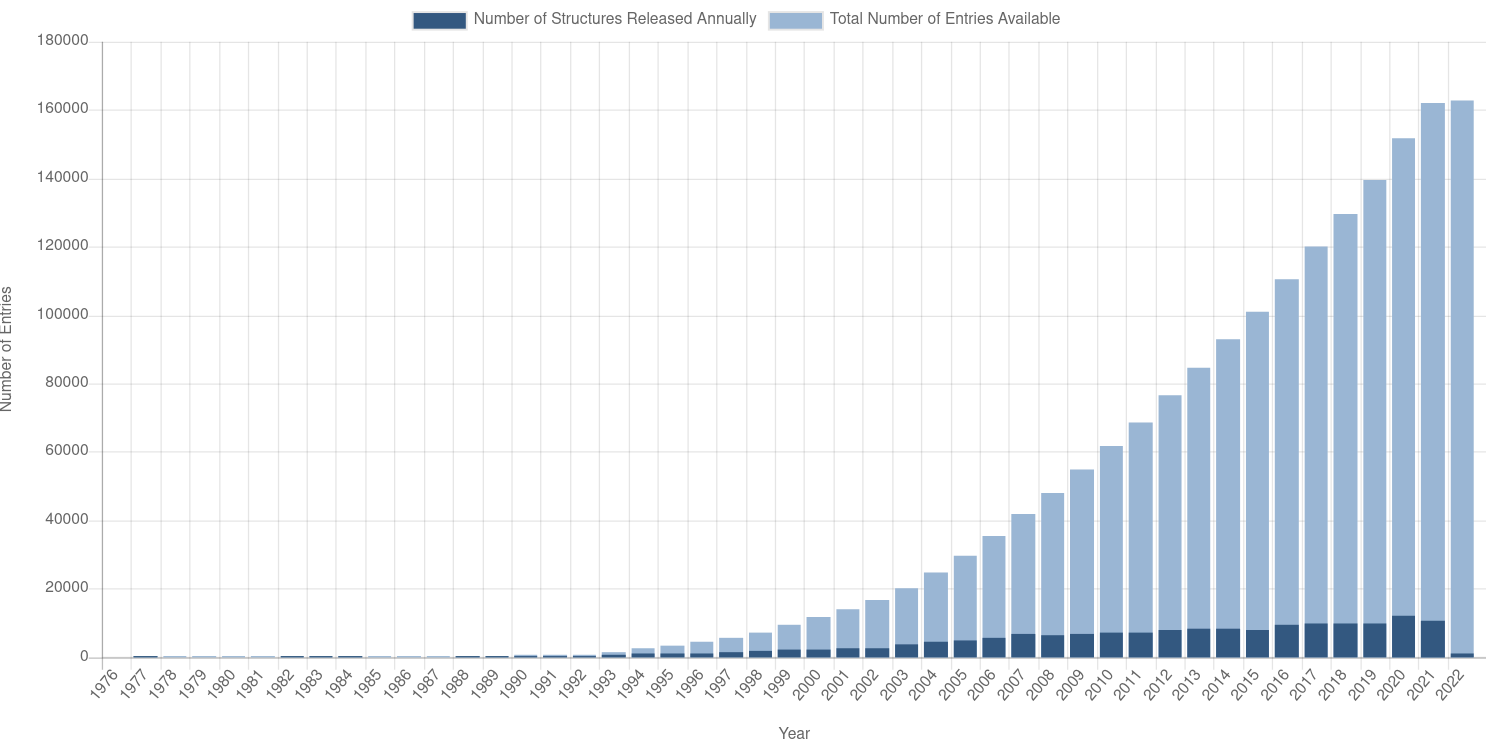
\includegraphics[scale=0.3]{images/pdb-statistica.png}
	\caption{Crescita complessiva del numero di strutture di proteine pubblicate nel PDB. Fonte\cite{pdbStats}}
	\label{fig:pdb-statistica}
\end{figure}


\section{Metodi e strumenti informatici}
La piccola percentuale di strutture determinate e il gap che continua a crescere con le sequenze conosciute è una conseguenza della lentezza e della dispendiosità dei metodi sperimentali (in parte anche dei progressi delle tecnologie di sequenziamento). I metodi computazionali, significativamente più veloci ed economici, potrebbero fornire una possibile soluzione a questo problema.

\subsection{Paradigmi per approssimazione biologica}
kessel 3.4 [computational methods for structure prediction]
pal 15.3.2 Computational structure prediction. Molto breve
pal 18.1 [molecular dynamics]
psp-wiki [abbastanza discorsivo]
prot-eng-wiki[molto breve]
Gu 28-33 [serie di articoli messi insieme, sembra stra interessante]
baxevanis 12 p.385 \\ \\

I numerosi metodi computazionali per il PSP\footnote{Le sezioni sui paradigmi per approssimazione biologica seguono e si basano in larga parte sul capitolo 3.4 di \fullcite{kessel_ben-tal_2018}} possono essere suddivsi in base all'utilizzo o meno di informazioni prese da template (proteine con struttura 3D nota)\supercite{wei2019protein}:

\begin{itemize}
	\item metodi \textit{template-free}:
	
	\begin{itemize}
		\item \textit{ab initio} (o \textit{de novo}), approccio fisico, nel quale la struttura è predetta da zero in base a principi fisici (viene simulato un campo di forza)
		\item \textit{fragment-based}, in cui i calcoli sono realizzati su piccoli frammenti della proteina invece che sulla sua interezza
		\item \textit{knwoledge-based}, il campo di forza è sostituito da una funzione di valutazione
		\item \textit{correlated mutation} (o covariazione evolutiva), nel quale vengono inferiti contatti fra residui identificando mutazioni in risposta ad altre mutazioni
	\end{itemize}
	
	\item metodi \textit{template-based}:
	\begin{itemize}
		\item \textit{homology modeling}, basato su confronti sequenza-sequenza tra la proteina da predire e il modello
		\item \textit{fold recognition}, basato su altre similitudini fra modello e proteina target come la formazione di strutture secondarie
	\end{itemize}

\end{itemize}

Come si vedrà analizzando ogni approccio in dettaglio nelle sezioni \ref{sec:template-free} e \ref{sec:template-based}, ognuno presenta svantaggi e vantaggi, pertanto i metodi migliori sono quelli che combinano varie tecniche a seconda del caso (vedi sez. \ref{sec:metodi-integrativi} sui metodi integrativi).

\subsection{Paradigmi nel soft computing}
\subsubsection{ANN, EC, SVM, .. [..]}
\subsubsection{altri approcci [..]}

\subsection{Database e rappresentazione delle informazioni}
pal 6.4.1 p.145
Gu 10-13 p.468
baxevanis 12 p.367

\subsubsection{Database}
baxevanis 12 p.373, 1

\subsection{Visualizzazione grafica}
pal 6.4 p.146, ottima
kessel p.174 (2.3 GRAPHIC REPRESENTATIONS OF PROTEINS)

\subsection{CASP}
-abbass 2020

\section{Workflow nel PSP}
- paper Soft computing
- wiki psp

\subsection{Input, output, valutazione}
\subsubsection{Proprietà dei dati di input}

\subsubsection{Output: modelli, ... [..]}
\subsubsection{Metriche di valutazione}
- Gu 16 p.655 GENERAL APPROACH TO STRUCTURE COMPARISON AND ALIGNMENT
baxevanis 12 p.386

\section{Approcci \textit{template-free}} \label{sec:template-free}

\subsection{\textit{ab initio}}
{
Il metodo più lineare e a prima vista ovvio per predire la struttura nativa di proteine è seguire la natura, simulando accuratamente come le forze fisiche guidino la proteina a ripiegarsi e usare questa simulazione per riprodurre il processo di ripiegamento su proteine con strutture sconosciute. \textit{Ab initio}, termine latino, significa infatti "dall'inizio". Questo approccio si basa sul postulato di Anfinsen.

\par Il primo problema che sorge è superare il paradosso di Levinthal. Per farlo si assume un profilo energetico a imbuto del ripiegamento, ovvero la premessa termodinamica che la forma nativa di una proteina sia lo stato in cui risulta avere più bassa energia libera, o più precisamente (richiamando la definizione di struttura nativa data nella sez. \ref{sec:energetica}) quella conformazione avente minore energia libera tale da mantenere il livello di dinamicità richiesto alla proteina per svolgere la sua funzione biologica.

\par Le predizioni nell'approccio \textit{ab initio} sono pertanto \textit{energy-based}, ovvero guidate dall'idea di minimizzare l'energia. Si può vedere il PSP secondo l'approccio \textit{ab initio} come un problema di ottimizzazione dove una funzione di energia gioca il ruolo di \textit{euristica} cercando di raggiungere il minimo globale di energia all'interno dello spazio di ricerca. In quanto \textit{energy-based} usano solo informazioni sul tipo di atomi nel sistema, le loro posizioni relative nello spazio tridimensionale e le loro interazioni con gli altri atomi. Viene poi calcolato l'intero contenuto di energia del sistema e le forze agenti su ogni atomo. 

\par L'energia totale di un sistema (\textit{free energy}) può essere decomposta in varie componenti: cinetica, potenziale, termica ecc. È l'energia libera che determina la stabilità del sistema. Come si vedrà sotto, nell'approccio fisico non viene calcolata tutta l'energia libera ma solamente approssimata con una parte di essa per motivi di complessità.

\par Sebbene vi siano differenti metodi in questo approccio, tutti condividono due caratteristiche di base:
\begin{itemize}
	\item calcolano il contenuto di energia del sistema in una singola configurazione
	\item campionano numerose configurazioni e ne trovano una con la minor energia libera
\end{itemize}

Per \textit{configurazione} si intende la disposizione complessiva di tutti gli atomi di tutti i componenti del sistema (proteina, solvente, ioni, membrana ecc.) mentre la posizione collettiva dei soli atomi della proteina viene chiamata \textit{conformazione}.

\subsection{Molecular mechanics \& dynamics}

\par Per descrivere in maniera affidabile tutte le forze fisiche operanti sul sistema tra i differenti atomi bisognerebbe descriverne la distribuzione di tutti gli elettroni, il che richiede però calcoli di meccanica quantistica (QM). Le forze, in un sistema molecolare, risultano dalla distribuzione spaziale degli elettroni attorno agli atomi. Sfortunatamente questi calcoli sono computazionalmente molto costosi e una rigorosa caratterizzazione di un sistema macromolecolare, con milioni di atomi, è al momento insostenibile. Calcoli di QM su una singola conformazione di una piccola proteina possono richiedere mesi, tempi troppo lunghi se si ha l'obiettivo di provare tante configurazioni per sceglierne una finale. 

\subsubsection{Molecular mechanics}

\par Per le ragioni sopra elencate gli scienziati spesso investigano sistemi macromolecolari usando approssimazioni delle reali forze in essi. Il campo da cui i calcoli per le approssimazioni sono presi è chiamato \textit{molecular mechanics} (MM), poiché approssima sistemi molecolari usando espressioni prese dalla meccanica newtoniana classica:
\begin{itemize}
	\item il contenuto di energia è descritto usando un \textit{campo di forza} nel quale gli atomi e i legami covalenti sono trattati come palline e molle
	\item le descrizioni che richiederebbero calcoli di QM vengono ignorate
	\item le rappresentazioni sono \textit{esplicite}: prendono in considerazione tutti gli atomi (vedi fig. \ref{fig:descrizione-esplicita-mm})
\end{itemize}

Il campo di forza sopra accennato descrive l'energia potenziale del sistema. Da notare che l'energia potenziale (intesa come entalpia) è solo una delle due componenti dell'energia libera, vedi sez. \ref{sec:energetica}).

\par Un campo di forza è un'energia di posizione: l'energia di un oggetto in una specifica posizione all'interno di un campo (gravitazionale, elettrico, magnetico ecc.). Nelle molecole l'energia potenziale è la somma di tutti gli effetti dei campi elettrici atomici\footnote{gli atomi possiedono, in base alla loro eventuale carica, campi elettrici che influenzano gli altri atomi} in una determinata posizione. Si può approssimare l'energia potenziale all'energia risultante da tutti i legami covalenti e le interazioni non covalenti, escluse quelle non polari \footnote{un esempio di interazione non polare è l'effetto idrofobico. Vengono escluse poiché coinvolgono principalmente cambiamenti di entropia nel solvente}, in una singola configurazione del sistema.

\begin{figure}[!htb]
	\centering
	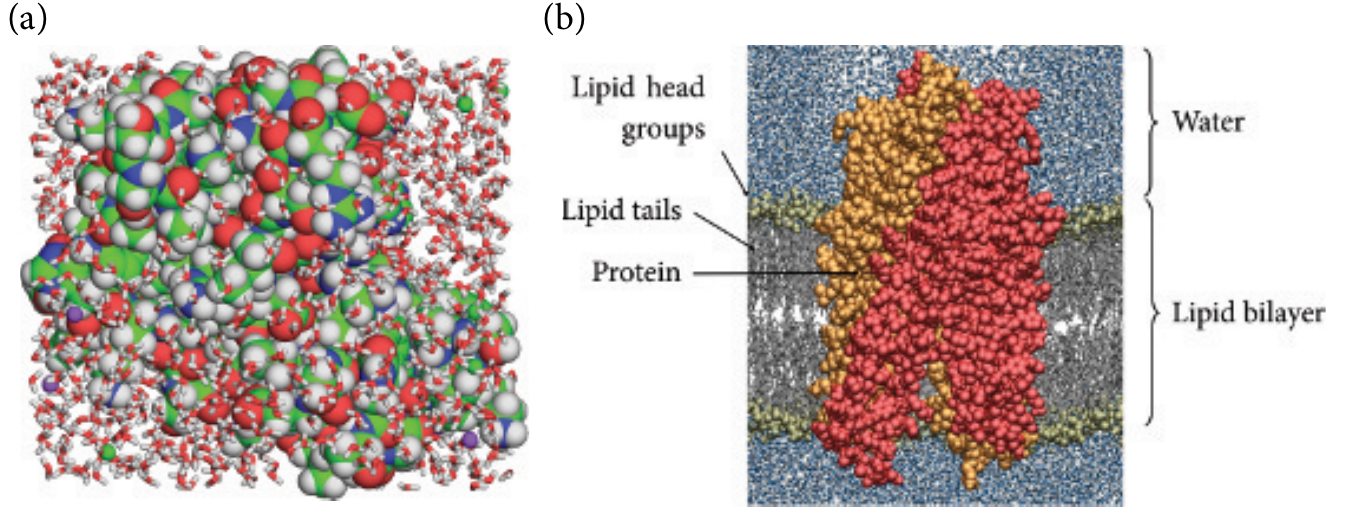
\includegraphics[scale=0.4]{images/esplicita-mm.png}
	\caption{Descrizioni esplicite nei calcoli di MM. (A) una piccola proteina immersa in un solvente composto da molecole d'acqua e ioni (Na$^{+}$, Cl$^{-}$). La proteina è rappresentata come sfere di atomi, l'acqua come bastoncini e gli ioni come piccole sfere magenta e gialle. (B) una proteina trasportatrice in un doppio strato lipidico, circondato da ambiente acquoso. La proteina e le teste dei lipidi sono rappresentate in modo space-fill, mentre l'acqua e le code dei lipidi con rappresentazione wire-frame. Fonte \cite{kessel_ben-tal_2018}}
	\label{fig:descrizione-esplicita-mm}
\end{figure}

\par La descrizione approssimata fornita dal campo di forza permette di calcolare l'energia potenziale di molti sistemi macromolecolari in meno di un secondo. \\

\par Una variante del MM è la \textit{QM/MM} nella quale i calcoli di QM sono indirizzati solamente su una piccola parte della proteina che contiene residui funzionali importanti. Le altre regioni sono soggette invece a MM, con calcoli molto più veloci \footnote{questo approccio è stato introdotto da Warshel, Levitt e Karplus}

\subsubsection{Spazio configurazionale}

\par Assumendo l'accuratezza del campo di forza, il calcolo dell'energia potenziale di un sistema consente di determinare (parte del)la stabilità di una configurazione. L'idea iniziale potrebbe essere quella di considerare tutte le possibili locazioni atomiche del sistema, calcolare l'energia potenziale in ogni caso e scegliere quella con la minor energia. Come si può facilmente intuire ciò risulta essere un procedimento troppo oneroso, in quanto si devono considerare anche gli atomi del solvente (ed eventuali ligandi o cofattori). Anche il solo numero delle possibili configurazioni atomiche è difficile da calcolare.

\par Per superare questo problema vengono usate tecniche per ridurre lo spazio di ricerca nello spazio configurazionale. Ci sono vari metodi di ricerca, ad esempio: \textit{systematic search }(grid search basata su dettagli geometrici), \textit{model-building model }(usa frammenti molecolari), \textit{random approach }(movimenti random sul piano cartesiano da una configurazione iniziale), \textit{distance geometry} (usa una matrice di distanze atomiche), \textit{Monte Carlo method} (modifiche random e accettazione probabilistica di configurazioni a livelli energetici maggiori)\supercite{ROY2015151}.

\par Il metodo più semplice è chiamato \textit{energy minimization}:

\begin{enumerate}
	\item si parte da una configurazione arbitraria
	\item si calcola l'energia potenziale. Viene derivato questo valore su differenti posizioni nel sistema in modo da calcolare le forze agenti su ogni atomo dalla rimanente parte del sistema
	\item un piccolo cambiamento è introdotto nella posizione di ogni atomo, in risposta alle forze applicate su ognuno di essi dal resto del sistema (in accordo a quanto calcolato nel precedente step)
	\item se la nuova configurazione ha un'energia minore viene adottata
	\item altrimenti questa viene scartata e viene creata una nuova configurazione
	\item si ritorna allo step 3 finché non si trovano più configurazioni con minor energia
\end{enumerate}

Il metodo passa da una configurazione all'altra scendendo con il gradiente della superficie dell'energia potenziale finché non converge in un \textit{punto di minimo locale}. Tutte le procedure di \textit{energy minimization }tendono a rimanere bloccate in un minimo locale di energia non riuscendo spesso a raggiungere il minimo globale a causa di \textit{barriere energetiche} da scavalcare per raggiungere una configurazione con energia minore (vedi fig. \ref{fig:energy-minimization} e \ref{fig:imbuto}).

\begin{figure}[!htb]
	\centering
	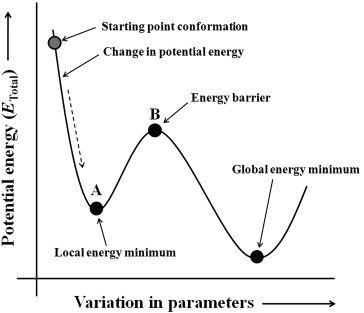
\includegraphics[scale=1]{images/energy-minimzation.jpg}
	\caption{Differenti fasi energetiche di una molecola durante la sua minimizzazione energetica. Fonte\cite{ROY2015151}}
	\label{fig:energy-minimization}
\end{figure}

\subsubsection{Molecular dynamics}

È possibile spingere l'algoritmo di minimizzazione energetica fuori da punti di minimo locale fornendo energia extra, ad esempio innalzando la temperatura del sistema (ovvero aggiungendo calore virtuale). L'energia aggiunta consente agli atomi del sistema di incrementare i loro movimenti e nuove configurazioni fuori dalle barriere energetiche vengono create. Questo metodo è chiamato \textit{Molecular dynamics} (MD) e si focalizza sui movimenti dipendenti dal tempo degli atomi nel sistema. I calcoli sono realizzati in accordo alla meccanica classica. 

\par Agli atomi viene assegnata una velocità iniziale (proporzionale alla temperatura) e continuano a muoversi nello spazio secondo i corrispondenti cambiamenti nell'energia potenziale del sistema. Il movimento di ogni atomo nel sistema è calcolato in base alla sua energia in quel dato momento.

\par Le simulazione di MD sono eseguite in cicli ripetitivi di \textit{riscaldamento} e \textit{raffreddamento} (metodo conosciuto nel mondo informatico come \textit{simulated annealing}, in riferimento al processo di tempra dei metalli). Nella fase di riscaldamento vengono superate le barriere energetiche mentre la fase di raffreddamento (seguita dall'\textit{energy minimization}) consente al sistema di rilassarsi in configurazioni con minor energia.

\par Un metodo comune per rendere la ricerca con MD più efficiente è di spezzarla in due fasi:
\begin{itemize}
	\item ricerca a bassa risoluzione per trovare una collezione di strutture con interazioni non polari (basato sulla nozione che il nucleo delle proteine globulari sia idrofobico)
	\item ricerca ad alta risoluzione fra le strutture selezionate nel primo step
\end{itemize}

\subsubsection{Limiti dell'approccio fisico e parziali soluzioni}
Sebbene simulare il ripiegamento proteico seguendo la meccanica classica possa apparire un approccio attraente, questo è pratico solo per piccole proteine e usando alte risorse computazionali: lo spazio di ricerca è enorme e il problema è computazionalmente intrattabile in modo deterministico (è NP-hard)\supercite{abbass2020enhancing}.

\par I metodi di MM/MD trovano difficilmente impiego in processi biologici rilevanti come il protein folding. Alcuni problemi riguardano l'approssimazione in sé del campo di forza, la sua accuratezza e i possibili doppi conteggi delle forze in gioco (es. interazioni ioniche e legami idrogeno calcolate in due espressioni differenti). 

\par Un altro problema, sempre nell'approssimazione dell'energia libera con campi di forza, è che forniscono sì l'energia potenziale ma non l'entropia. L'unico modo per stimare l'entropia e l'energia libera dai calcoli per l'energia potenziale è eseguire questi calcoli su tutte le possibili configurazioni del sistema e poi integrarli. Il problema risiede quindi nell'impossibilità di compiere la totalità di questi calcoli a causa delle rappresentazioni esplicite usate nelle simulazioni di MD. In particolare è difficile considerare tutte le configurazioni del solvente acquoso. Ciò che si sta calcolando non è l'energia libera ma un \textit{potenziale di forze medie} (PMF). In conclusione le simulazioni di MD non sono consigliate per descrivere gli effetti dei solventi.

\subsubsection{Mean field approach}
Per ovviare parzialmente al problema delle rappresentazioni esplicite è possibile descrivere \textit{implicitamente} parti del sistema che vengono descritte da una proprietà media, per questa ragione tale approccio è chiamato \textit{mean field}. Un esempio è la descrizione del solvente, la parte "meno" interessante in genere, come una massa omogenea descritta dalla sua \textit{dielettricità} \footnote{proprietà di un mezzo non conduttore di essere sede di un campo elettrostatico}, conosciuto anche come approccio \textit{continuum-solvent}, vedi fig. \ref{fig:mean-field}.

\begin{figure}[!htb]
	\centering
	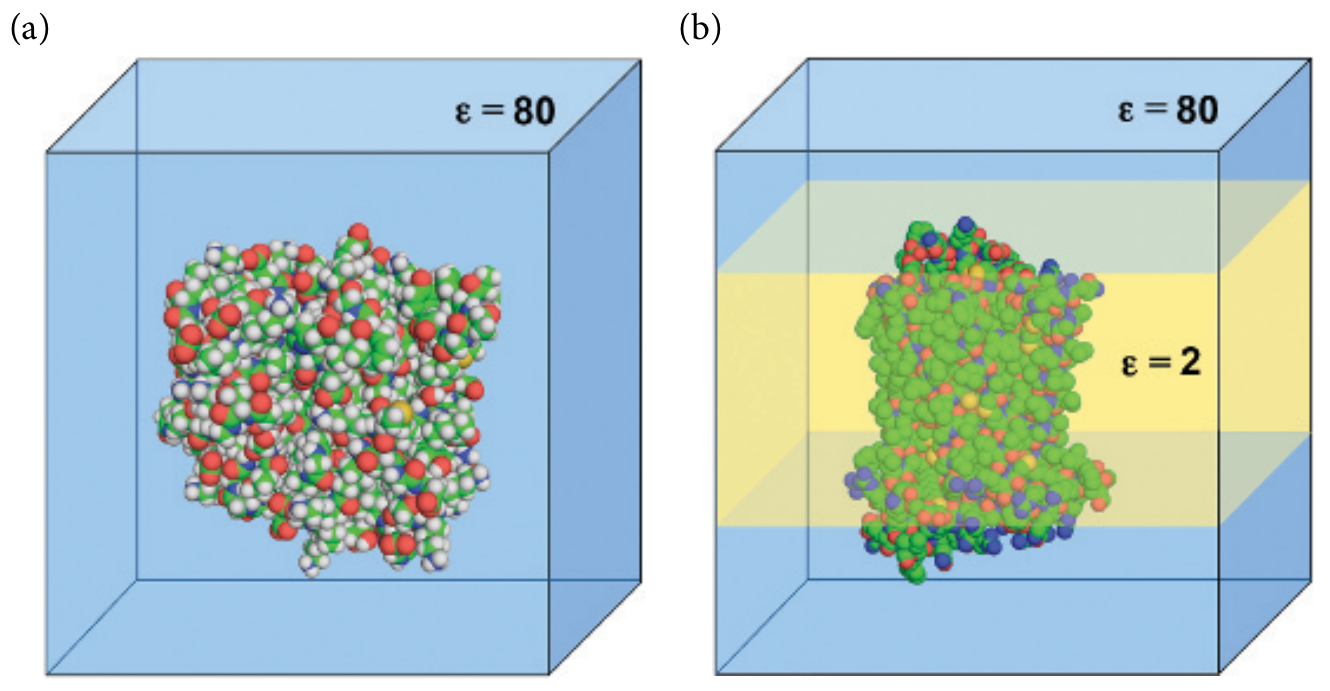
\includegraphics[scale=0.4]{images/mean-field.png}
	\caption{Descrizione con approccio mean-field di un sistema, il solvente è descritto implicitamente mentre la proteina esplicitamente. $\epsilon$ indica la dielettricità. (A) proteina in un solvente acquoso altamente dielettrico. (B) proteina di membrana in un ambiente eterogeneo. Il solvente acquoso è altamente dielettrico mentre la lastra semi-trasparente gialla, che rappresenta la regione biologica di doppio strato lipidico, è poco dielettrica. Fonte\cite{kessel_ben-tal_2018}}
	\label{fig:mean-field}
\end{figure}

Ovviamente, essendo una forte approssimazione, alcuni aspetti del sistema reale sono ignorati, come le interazioni fra gli atomi delle proteine e le molecole d'acqua. Tale problema si esacerba quando il solvente è una membrana. \\

\par Un altro compromesso è l'approccio \textit{mixed force fields} che combina calcoli espliciti sulla proteina e calcoli impliciti sul solvente. Viene usata l'equazione di Poisson-Boltzman (PBE) per calcolare accuratamente l'energia libera elettrostatica, legando così l'effetto polarizzante delle cariche con il loro ambiente. Essendo però un calcolo oneroso viene in genere risolta l'equazione generalizzata di Born (GB). A partire da queste due equazioni, che calcolano la componente elettrostatica dell'energia libera, è possibile calcolare l'intera \textit{free energy}, in modo abbastanza accurato, con calcoli che si rifanno alla surface area (SA, vedi parte finale della sez. \ref{sec:termodinamica-forze-idrofobiche}). 

\par Questi metodi sono chiamati \textit{PBSA} e \textit{GBSA} rispettivamente, e come si è visto permettono un calcolo più preciso dell'energia libera. Questi possono a loro volta essere combinati con la MM per rappresentare anche le interazioni del sistema (\textit{MM-PBSA, MM-GBSA}) e sono oggi largamente utilizzati.

\par Un altro limite computazionale è il lasso temporale che si riesce a coprire. La maggior parte delle proteine si ripiega in microsecondi mentre le simulazioni riescono a coprire tempi che vanno dai pico ai nanosecondi. Grazie ad avanzamenti nelle risorse informatiche sono stati fatti dei passi avanti da questo punto di vista. Un caso interessante è \textit{Anton}, un supercomputer progettato specificatamente per ottimizzare simulazioni di MD capace di coprire 85$\mu s$ al giorno per un sistema molecolare di 23.000 atomi (180 volte più veloce di qualsiasi computer general-purpose). Altri progressi sono dovuti alla computazione parallela e alla computazione accelerata dalla GPU. Il calcolo distribuito (\textit{grid computing}), ovvero una larga rete di computer personali dedicati volontariamente al completamento di processi, ha permesso alla rete \textit{Folding@Home} (170.000 computer) di simulare l'intero processo di ripiegamento della proteina di legame dell'acetil coenzima A, composta da 86 residui e che richiede 10 millisecondi per ripiegarsi. Un'altra rete distribuita di calcolo è \textit{Rosetta@Home}, con 86.000 nodi e finalizzata al PSP. \\

\subsubsection{Conclusioni sull'approccio \textit{ab initio}}
I metodi \textit{ab initio} non sono attualmente in grado di predire la struttura della maggior parte delle proteine sulla sola base della loro sequenza. Ma sono molto abili nel farlo quando il punto di partenza della predizione è una struttura vicino a quella nativa. Questi metodi sono infatti ampiamente usati per raffinare le strutture grezze ottenute dalle determinazioni sperimentali (vedi sez. \ref{sec:experimentally-guided-prediction}). 

\par Il loro successo dipende ampiamente dall'accuratezza della funzione di energia, dall'efficienza dell'algoritmo di ricerca nello spazio conformazionale e dall'abilità di discernere strutture native da "esche" energeticamente intrappolate.
Nonostante le loro limitazioni i metodi \textit{ab initio} sono di grande interesse perché sono gli unici, in principio, derivare la vera struttura nativa delle proteine e possono quindi fornire intuizioni importanti per il protein folding problem. Hanno infatti fornito informazioni importanti sulla dinamica delle proteine e sono utilizzati anche nel \textit{protein engineering} e nel \textit{drug discovery}. 

}


\subsubsection{Valutazione \textit{knowledge-based}}
\par È anche possibile rimpiazzare il campo di forza con una funzione di valutazione \textit{knowledge-based}. Spesso queste funzioni sono composte di espressioni relative alla tendenza statistica di gruppi chimici, amminoacidi o atomi di interagire fra di loro. L'affidabilità della funzione di valutazione dipende dal database su cui si basa. 


\subsection{\textit{correlated mutation}}


Such analysis infers spatial proximity by
detecting mutations that occurred in the
same evolutionary timeframes in response
to other mutations.

L'approccio per coevoluzione evolutiva può essere combinato con l'approccio \textit{template-based}, come dimostra AWSEM\supercite{jin2020protein} nella 13° edizione del CASP, il quale contiene anche metodi di ottimizzazione di energia e utilizzo di reti neurali.


\subsection{\textit{fragment-based}}
\par Un possibile metodo di azione è la \textit{frammentazione delle proteine}, nel quale i calcoli sono realizzati su piccoli frammenti della proteina e poi integrati. Un esempio è il software QUARK. L'approccio \textit{fragment-based} è usato nei metodi che combinano predizioni \textit{template-based} con assemblaggi \textit{ab initio}.


fragment-based
assembly is the dominant technique due to
its higher accuracy and higher capability
whenever a good template is difficult to



Wang et al.’s DeepFragLib advances
the field by introducing deep learning
to another central component of protein
structure prediction: protein-specific
fragment libraries.

These libraries are
prebuilt databases for assembling proteins.
The efficient assembly of near-native
conformations relies on high-quality,
native-like fragments for every segment of
a protein.



\section{Approcci \textit{template-based}} \label{sec:template-based}
Le proteine che esistono in natura oggi si sono sviluppate attraverso lunghi processi evoluzionistici, progredendo attraverso mutazioni casuali e selezione naturale. La rivoluzione genetica degli anni '50, consentendo la determinazione delle sequenze amminoacidiche, ha permesso il nascere di metodi di confronto delle sequenze. Si possono ricavare informazioni sulla struttura 3D delle proteine cercando altre proteine con proprietà nella sequenza simili e una struttura nota, ovvero dei \textit{template}. 

\subsection{\textit{homology modeling}}
{
Nella modellazione per omologia ci si affida a somiglianze nella sequenza tra la proteina target e i template. I metodi per omologia sono perciò basati sul paradigma: \\
 \say{\textit{la sequenza codifica per la struttura}}.

\par Sono metodi basati anche sull'osservazione che la struttura terziaria è più conservata della sequenza amminoacidica. Di conseguenza ci si aspetta una significativa somiglianza nella struttura fra proteine che condividono una notevole somiglianza tra le sequenze, anche non totale.

\par In altri termini, due sequenze amminoacidiche molto simili (\textit{omologhe}) , in due proteine differenti ma evoluzionisticamente collegate, dovrebbero acquisire la stessa struttura locale.

\par La modellazione per omologia consiste tipicamente nei seguenti passi:
\begin{enumerate}
	\item ricerca e selezione del template
	\item costruire un MSA (Multiple Sequence Alignment) che includa la proteina target e i template
	\item assegnare le coordinate spaziali dei template alla sequenza della proteina target
	\item raffinamento della struttura modello
	\item valutazione e validazione della struttura risultante
\end{enumerate}

\begin{figure}[!htb]
	\minipage{0.48\textwidth}
	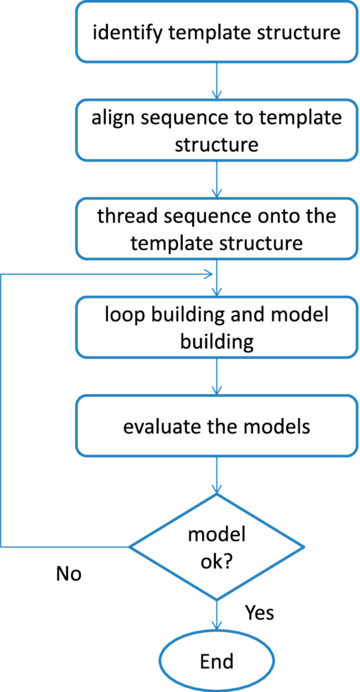
\includegraphics[scale=0.43]{images/homology1.png}
	\caption{Diagramma di flusso della modellazione per omologia. Fonte: \cite{sliwoski2014computational}}
	\label{fig:omologia-flusso}
	\endminipage\hfill
	\minipage{0.48\textwidth}
	\centering
	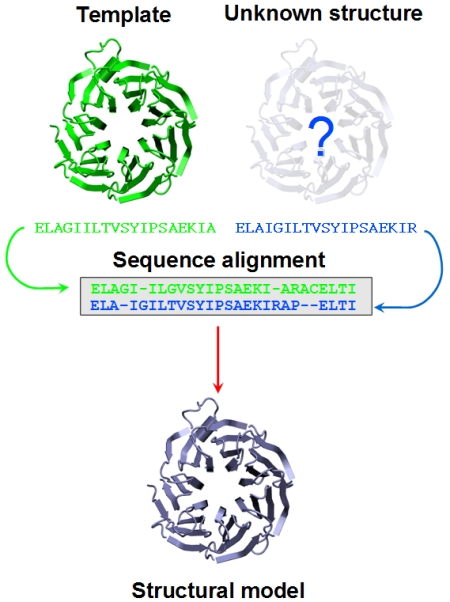
\includegraphics[scale=0.5]{images/homology2.jpg}
	\caption{Schema esemplificativo di una modellazione per omologia. Fonte \cite{UNIL-homology}}
	\label{fig:omologia-esempio}
	\endminipage\hfill
\end{figure}

Nel 1° step si cerca una struttura modello, almeno una, tra le strutture conosciute avente un'alta somiglianza di sequenza. È più semplice se la struttura di un una proteina omologa molto simile è stata già risolta. Ci sono però altri gruppi di proteine, come le proteine di membrana, le cui strutture risolte sono scarse. Trovare i giusti template e caratterizzare la loro omologia è ciò che determina in genere il successo dell'intera predizione (una somiglianza minore del 30\% avrà risultati molto scarsi, mentre sopra al 50\% la predizione ha buona probabilità di essere di buon livello). È possibile in ogni caso che vi sia una somiglianza \textit{locale} anche quando la somiglianza globale è scarsa. Le principali tecniche si dividono nelle seguenti categorie:
\begin{itemize}
	\item pattern recognition e ricerche euristiche, ad esempio BLAST (Basic Local Alignment Search Tool) e FastA
	\item profile and iterative alignment methods, come PSI-BLAST e HMM (Hidden Markov Models), quest'ultimo molto usato
	\item structure based threading, come THREADER e FUGUE
\end{itemize}

\par Nel 2° step vengono sfruttate informazioni evoluzionistiche per migliorare l'allineamento tra le sequenze dei template e del target. È difficile stabilire allineamenti fra omologhi distanti, come nel caso di target \textit{eucarioti} e template \textit{procarioti}. La tecnica più usata oggi è l'MSA, altre tecniche usate sono: programmazione dinamica, MSA, threading, HMM ecc. Ci sono vari tool per creare MSA, ad esempio: Clustal$\Omega$, MAFFT, MUSCLE, T-Coffee. Possono venire utilizzati più MSA insieme per sopperire a problemi di disallineamento di piccole regioni. Il MSA viene illsutrato dopo la sezione \ref{sec:MSA}.

\par Nel 3° step ad ogni segmento della sequenza target viene assegnato un insieme di coordinate spaziali in accordo ai risultati del MSA. Tool noti sono MODELLER (soddisfazione di vincoli spaziali), NEST, COMPOSER e SWISS-Model. La struttura ottenuta potrebbe essere però deformata a causa dell'utilizzo di più template e numerosi inserzioni e cancellazioni. Possono essere presenti lunghezze e angoli dei legami non ottimali e atomi sovrapposti.

\par Per ovviare a tali problemi nello step 4 si applica un processo di raffinamento, specialmente per quanto riguarda i loop (\textit{loop modeling}, vedi sez. \ref{sec: loop-modeling}), regioni fodamentali per i siti di legame, e i residui (\textit{side chain modeling}). Vengono applicati algoritmi che confrontano caratteristiche geometriche ed effettuano calcoli energetici che identificano configurazioni atomiche sfavorevoli. 

\par Nel 5° step si valuta l'affidabilità della predizione. Si dice che un modello è affidabile in generale quando è basato su un template corretto e un allineamento approssimativamente corretto. Si può valutare tale affidabilità in vari modi:

\begin{itemize}
	\item alcune qualità della struttura costruita possono essere confrontate con delle tendenze statistiche 
	\item se ci sono vari modelli predetti si calcola l'energia libera e si sceglie la struttura con minor energia libera (ad es. tramite ProSa)
	\item stereochimica (relativa alle proprietà spaziali delle molecole), ad esempio con PROCHECK
	\item la conservazione evoluzionistica a livello amminoacidico può essere correlata con il loro stato "esposto" o "seppellito" (l'idea di partenza è che il nucleo della proteina rimanga inalterato e la superficie sia variabile), ad esempio Profiles3D
	\item se si hanno a disposizione dati sperimentali della struttura nativa della proteina si può validare il modello con la consistenza a essi.
\end{itemize}

\subsubsection{Efficienza e limiti}

Con una somiglianza maggiore del 50\% si registra una RMSD che tra 1 e 2 \angstrom, ma è importante notare che non sempre proteine omologhe (vicine sequenzialmente) condividono la stessa funzione e struttura. Un esempio sono le proteine del lievito Gal1 e Gal3: 73\% di identità e 92\% di somiglianza. Queste due proteine hanno però sviluppato differenti funzioni, con Gal1 che è una galattochinasi mentre Gal3 è un induttore trascrizionale\supercite{platt2000insertion}.

\par Non c'è quindi una soglia che assicuri una sicura predizione della struttura: molte proteine con una lontana somiglianza possono svolgere la stessa funzione mentre altre altamente simili possono svolgere funzioni diverse. Una regola empirica è considerare sequenze con più del 30-40\% di somiglianza come sequenze con una struttura o funzione simile.

\begin{figure}[!htb]
	\centering
	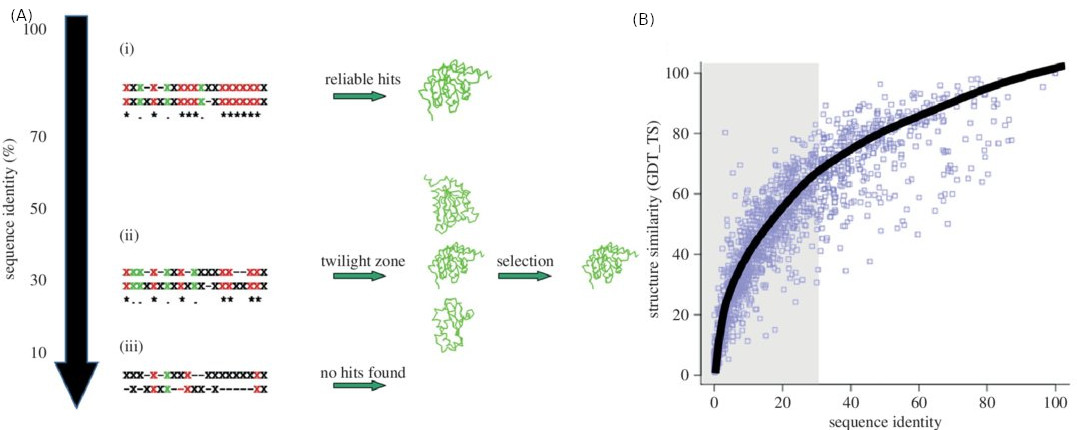
\includegraphics[scale=1.2]{images/homology-grafico.jpg}
	\caption{Risultati dei metodi per omologia alla variazione dell'identità nella sequenza. (A) Dimostrazione schematica dell'uso di confronti di sequenze per identificare omologie strutturali. 'X' indica un qualsiasi amminoacido. (i) identità > 70\%: semplici allineamenti di sequenza sono sufficienti per trovare il corretto ripiegamento. (ii) Tra il 20 e il 30\% non sempre è possibile trovare il corretto ripiegamento; è necessario effettuare ulteriori raffinamenti. (iii) a bassi livelli l'utilità di questo metodo è molto bassa. (B) Somiglianza strutturale (in GDT\_TS score) al variare dell'identità della sequenza. Anche al 30\% il livello di somiglianza è significativo. Fonte\cite{joseph2014local}}
	\label{fig:omologia-grafico}
\end{figure}

\par Un'osservazione fondamentale risiede sulle basi in sé del metodo: dato l'affidamento pressoché totale nella modellazione comparativa, la struttura modello è condizionata necessariamente a essere più simile ai template che alla reale struttura nativa della sequenza target, nonostante i vari processi successivi di raffinamento che, data la loro natura approssimativa, non sono perfetti. 

\par I problemi maggiori risultano nelle regioni con bassa somiglianza, come ci si può aspettare. Si sta parlando specialmente dei \textit{loop}, soggetti a mutazioni considerevoli durante l'evoluzione.

\par Si incorrono in problemi con la modellazione per omologia quando si trattano proteine che non hanno omologhe tra le strutture conosciute, come le proteine di membrana, le quali sono difficili da da cristallizzare. \\

\subsubsection{Conclusioni sulla \textit{modellazione per omologia}}

\par Nonostante tutte le osservazioni fatte, \textit{la modellazione per omologia è correntemente il miglior metodo computazionale per predire la struttura delle proteine} e la sua applicabilità è destinata a crescere con l'aggiunta di nuove strutture determinate sperimentalmente da poter essere usate come template.

\par La sfida principale che questi metodi hanno affrontato, e che AlphaFold ha "vinto", era raggiungere almeno una RMSD di 3\angstrom. Le sfide ancora da superare riguardano l'accuratezza su grandi proteine, su proteine con un contenuto significativo di strutture $\beta$ e la modellazione di proteine multi-dominio e di membrana.

\par Oltre alla PSP i metodi per omologia sono anche usati nel drug design (per studiare le differenze strutturali fra le proteine bersagliate dallo stesso farmaco) e nello studio dei meccanismi catalitici.

}

\subsection{Loop modeling} \label{sec: loop-modeling}

I loop sono regioni della struttura proteica con ruoli spesso cruciali (interazioni con altre proteine, siti di legame con molecole ecc.). Allo stesso tempo sono molto variabili nella loro sequenza e struttura rispetto alle altre regioni. Si trovano generalmente sulla superficie delle proteine e le loro strutture sono note per essere difficili da predire.

\begin{figure}[!htb]
	\minipage{0.48\textwidth}
	\centering
	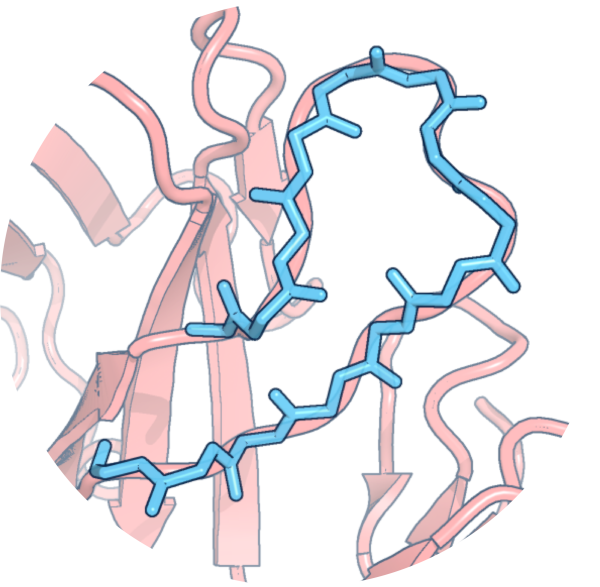
\includegraphics[scale= 1]{images/fread.png}
	\caption{Disegno di un loop in celeste. Fonte \cite{FREAD}}
	\label{fig:loop-example}
	\endminipage\hfill
	\minipage{0.5\textwidth}
	\centering
	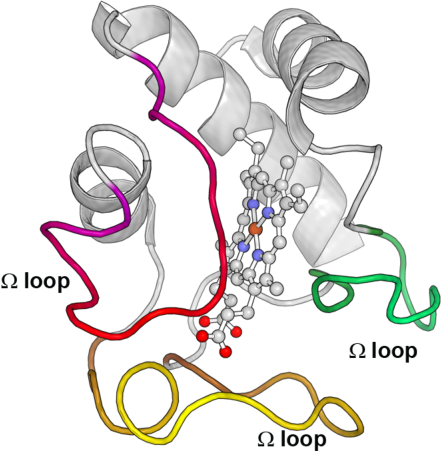
\includegraphics[scale=0.3]{images/loops.png}
	\caption{Omega loop. Sono spesso coinvolti nel riconoscimento molecolare e in funzioni regolatrici. Fonte: \cite{Papaleo2016TheRO}}
	\label{fig:omega-loops}
	\endminipage\hfill
\end{figure}

Il loop modeling non si applica solamente alla fase di raffinamento della modellazione per omologia della predizione di strutture proteiche. È importante anche nella predizione di frammenti mancanti nelle strutture determinate sperimentalmente. È stato stimato che in più della metà delle struttura depositate nel PDB ci siano segmenti mancanti, spesso loop\supercite{karami2018dareus}.

\par Problemi comuni nel loop modeling sono: decidere quale regione del modello sarà un loop; trovare il corretto allineamento di regioni di ancoraggio; la modellazione in sé del loop; le conformazioni di loop multipli, ecc.

\par Nella modellazione per omologia (nel PSP) si registrano spesso grandi deviazioni dai template omologhi: la modellazione dei loop rimane un problema aperto nella modellazione per omologia della struttura delle proteine\supercite{karamiLoop}. Le principali strategie per il loop modeling sono
\begin{itemize}
	\item \textit{data-based} (o knowledge-based), basati sull'assunzione di similarità sequenza-struttura, ovvero che loop con sequenze simili hanno anche conformazioni simili
	\item \textit{ab initio}, in cui viene esplorato lo spazio conformazionale
\end{itemize}

La ricerca su database è efficiente per famiglie specifiche ma i loop più lunghi di 4 residui devono essere comunque ottimizzati. I residui ai fianchi della regione del loop sono chiamati residui di \textit{ancoràggio} e sono utilizzati per effettuare la ricerca nei database. ArchPRED ad esempio considera le strutture secondarie ai fianchi del loop mancante, il loro orientamento relativo e il numero di residui mancanti per identificare conformazioni del loop candidate. È possibile usare una funzione di valutazione basata sull'energia per valutare la modellazione dei loop, ad esempio basata sulla stereochimica (come in CHARMM). 

\par Molti dei metodi raggiungono ottimi risultati per la predizione dei loop su strutture sperimentali in ambienti esatti (ovvero strutture cristallizzate a cui mancano le regioni dei loop). Ma nei modelli per omologia non si è ancora riusciti a raggiungere buoni risultati\supercite{karami2018dareus}. 

\par I metodi \textit{ab initio} sono dipendenti dalle tecniche di ottimizzazione dell'energia e per questa ragione risultano essere lenti. Metodi \textit{ab initio} per il completamento della struttura cristallizzata allo stato dell'arte sono Rosetta-NGK e GalaxyLoop-PS2. CODA è un esempio di metodo ibrido che combina i due approcci nel loop modeling, così come Sphinx il quale prima esegue una ricerca data-based per trovare frammenti più corti del loop di interesse in modo da ottenere informazioni strutturali, successivamente applica metodi \textit{ab initio} per generare frammenti della corretta lunghezza. \\

\par Pochi metodi sono disponibili come web servers e quindi utilizzabili anche dai non esperti: GalaxyLoopPS2, LoopIng, Sphnix e DaReUS-Loop. Metodi locali sono invece MODELLER, Loopy, OSCAR-loop, Rosetta-NGK, LEAP e M-DISGro. Sono disponibili anche dei tool per la modellazione di loop specifici per gli anticorpi, come quelli offerti da SAbPred\footnote{Collezione di tool sviluppati da Oxford Protein Informatics Group (OPIG).}: Sphinx e FREAD (knowledge-based) che effettua una ricerca su database tenendo in considerazione i vincoli spaziali dei residui di ancoràggio.

\par Uno dei metodi più recenti e con migliori risultati è DaReUS-Loop, un approccio  \textit{data-based} che identifica loop candidati estraendoli dal completo insieme delle strutture conosciute del PDB. Il filtraggio dei candidati si basa su confronti di conformazioni locali profilo-profilo insieme a una valutazione fisico-chimica. Applicato ai dataset del CASP11 e CASP12 mostra significativi progressi nell'accuratezza della predizione dei loop e propone una misura di confidenza che correla bene con l'accuratezza effettiva dei loop. I loro autori mostrano anche che oltre il 50\% dei modelli ben riusciti sono derivati da proteine non correlate: ciò suggerisce che frammenti di proteine, sotto simili vincoli, tendono ad adottare simili strutture (oltre la mera omologia)\supercite{karami2018dareus}. 

\begin{figure}[!htb]
	\centering
	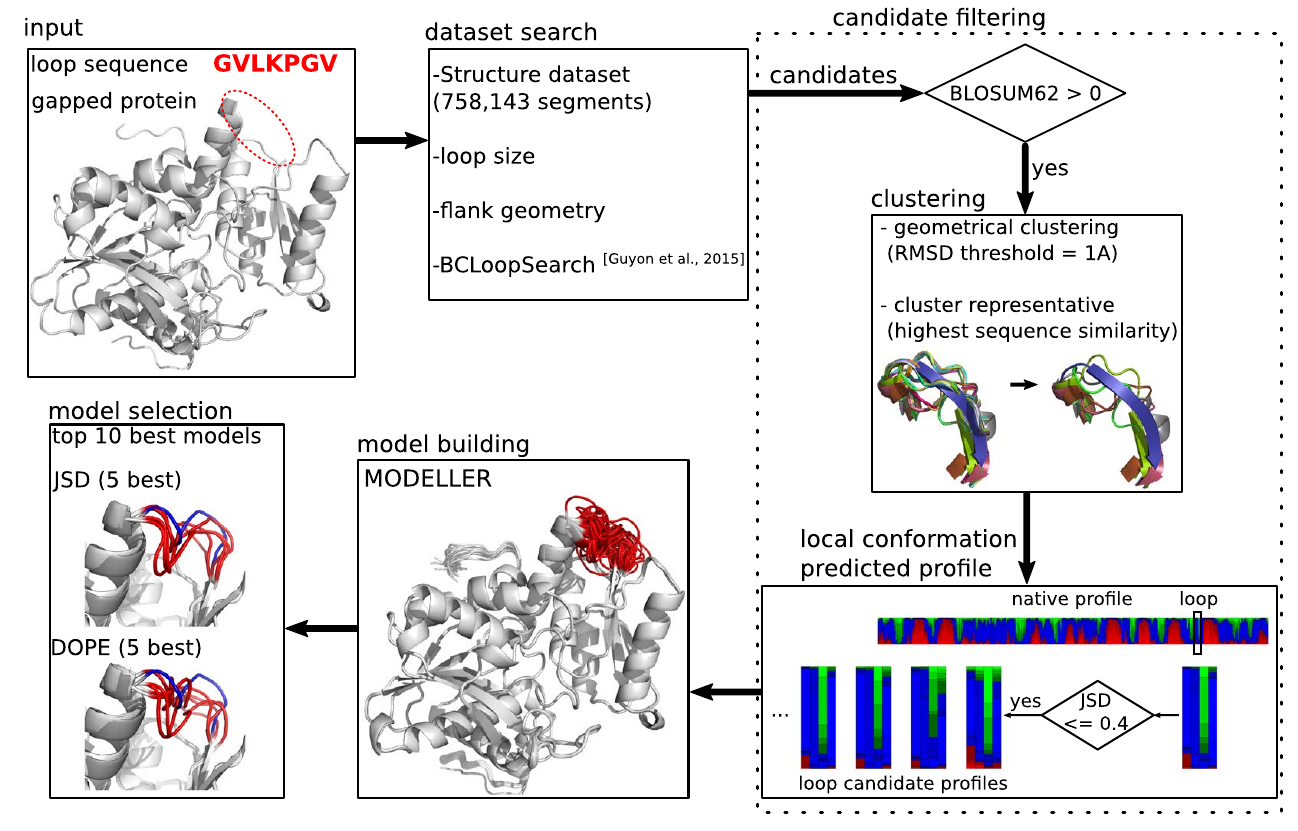
\includegraphics[scale=0.45]{images/dareus.png}
	\caption{DaReUS-Loop workflow. Da notare che dal 2019\supercite{karamiLoop} nel processo di costruzione del modello non è più usato MODELLER (non free) ma GROMACS. Fonte\cite{karami2018dareus}}
	\label{fig:dareus-workflow}
\end{figure}

I principali step del metodo sono mostrati in figura \ref{fig:dareus-workflow} e sono:
\begin{itemize}
	\item ricerca dei candidati del loop
	\item filtraggio dei candidati
	\item costruzione del modello
	\item model selection
\end{itemize}

Nell'ultimo step sono utilizzate 2 misure per valutare i modelli e vengono ritornati in output come predizioni finali i 5 migliori modelli per ogni metrica.

\begin{figure}[!htb]
	\centering
	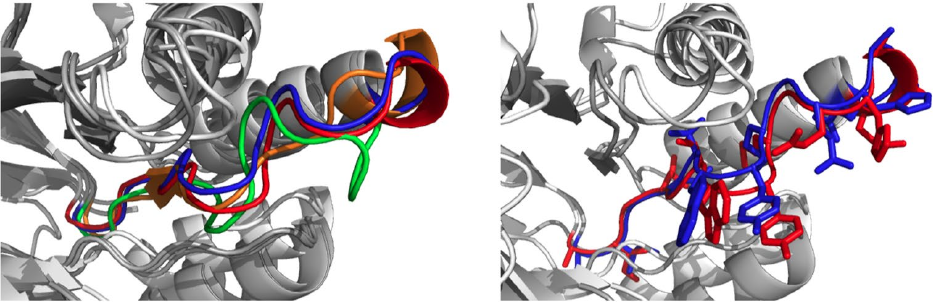
\includegraphics[scale=0.63]{images/dareus-confronto.png}
	\caption{Esempi di predizione di un loop lungo (15 residui) della proteina target T0807 del CASP11 a confronto. Blu=DaReUS-Loop, verde=Rosetta NGK, arancione=GalaxyLoop-PS2, rosso=struttura cristallizzata. La RMSD di ogni loop predetto rispetto al loop nativo è riportata di seguito. DaReUS-Loop: 1.3\angstrom, NGK: 3\angstrom, PS2: 2.9\angstrom. Nella colonna a destra sono riportate le catene laterali della struttura nativa e di quella predetta da DaReUS-Loop. Fonte\cite{karami2018dareus}}
	\label{fig:}
\end{figure}

\subsubsection{Sequence alignment} \label{sec:MSA}
- protein sequence alignment (poi MSA)
[Burkowski 6 p.167]
baxevanis 8 p.227


Certain software programs can display multiple sequences together to show the degree of similarity between them

This is called a sequence alignment and is commonly used to show the degree of relatedness between sequences

Le sequence di proteine in genere risultano avere un grado di somiglianza maggiore rispetto alle sequenze nucleotidiche, questo è dovuto alla degenerazione del codice genetico e al fatto che quasi per ogni amminoacido esistono vari codoni che lo codificano, perciò differenti sequenze nucleotidiche possono codificare esattamente la stessa sequenze di amminoacidi.

\begin{figure}[!htb]
	\centering
	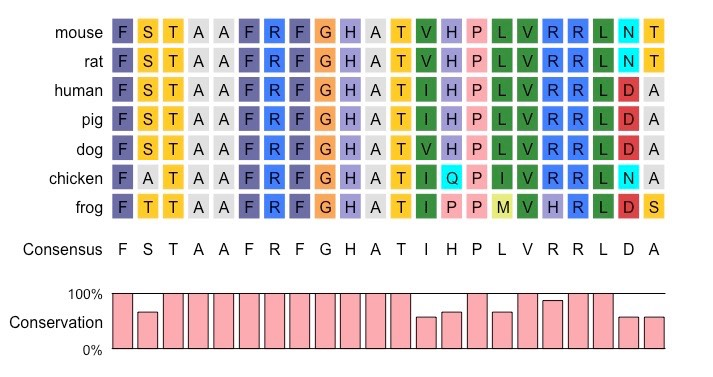
\includegraphics[scale=0.5]{images/msa.jpeg}
	\caption{Multiple sequence alignment schematica di una sequenza proteica di varie specie. Fonte\cite{msaBioNinja}}
	\label{fig:msa}
\end{figure}

\subsection{\textit{fold recognition} via \textit{threading}}
- praveen 2014
- pal 

Nei metodi per \textit{fold recognition} ci si basa su somiglianze nelle inclinazioni derivate dalla sequenza, come la formazione di strutture secondarie, o su tendenze statistiche.

\begin{figure}[!htb]
	\centering
	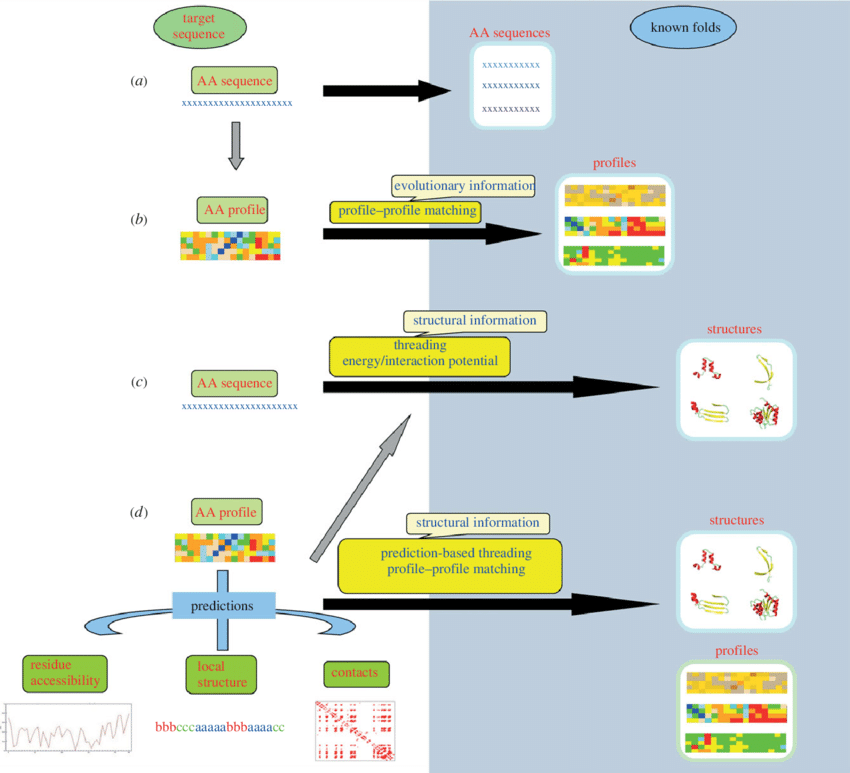
\includegraphics[scale=0.53]{images/threading-mappa.png}
	\caption{. Fonte\cite{joseph2014local}}
	\label{fig:fold-recognition}
\end{figure}


\subsection{Protein secondary structure prediction (PSSP)}
-wiki
-sejonwski 1989
-deOliveira 2021


\section{Metodi integrativi} \label{sec:metodi-integrativi}

- predictive methods
baxevanis 7

\subsection{Macromolecular docking??}


\section{Case Study: \textit{TASSER}}


\section{Determinazione sperimentale delle strutture} \label{sec:experimentally-guided-prediction}

La determinazione sperimentale della struttura delle proteine ha vissuto dei progressi significativi col passare degli anni ed è di grande importanza per i metodi computazionali di PSP.


- come le proteine sono studiate [alberts, 4.4 p.158]
- metodi sperimentali 
alberts p.168
pal 6 p.126 ma è molto tecnico
wiki-protein folding, 
baxevanis 12 p.363

• storia dei metodi sperimentali (Pal) \\
• cristallografia a raggi-x \\
• NMR, risonanza magnetica nucleare \\
• Cryo-EM (electron microscopy) \\

\section{Oltre la predizione di strutture sconosciute}

\subsection{Predizione guidata sperimentalmente}
kessel 3.5
pal 6.2.5 p.138

Anche quando gli scienziati hanno una proteina correttamente ripiegata fra le mani non è così semplice determinarne la sua esatta conformazione tridimensionale, considerando che si parla di strutture di migliaia di atomi.

Integrating experimental (i.e., lab) data with predictions [235]. Low-resolution
methods for the determination of protein structures (e.g., electron microscopy) have
recently been used for deriving geometric constraints, which can be applied along
with computational methods to achieve better predictions.

\subsection{Protein function prediction}
- pfp wiki

One should remember, though, that effi-
cient protein structure prediction is just a means to an end; the real challenge of structural
biology has always been (and still is) to deduce the functions of proteins on the basis of their
sequences and/or structural data [190].

Knowing the structure of a protein often allows functional prediction as well.

There is no hard sequence-similarity threshold for "safe" function prediction; many proteins of barely
detectable sequence similarity have the same function while others (such as Gal1 and Gal3) are highly
similar but have evolved different functions. 

For enzymes, predictions of specific functions are especially difficult, as they only need a few key residues
in their active site, hence very different sequences can have very similar activities. By contrast, even with
sequence identity of 70\% or greater, 10\% of any pair of enzymes have different substrates; and differences
in the actual enzymatic reactions are not uncommon near 50\% sequence identity.

\subsection{Drug design}
- sliwoski 2014
- isomorphic labs

\section{Storia della comprensione delle proteine}
- alberts p.160
- psp-wiki
- levitt 2001, birth of structural biology \\ \\


L'approccio \textit{ab initio} è emerso negli anni '60 a partire dal campo della chimica computazionale. Nel 2013 il premio Nobel per la chimica è stato assegnato proprio a quegli scienziati che hanno contribuito sin da quegli anni al campo della biofisica molecolare computazionale (Warshel, Levitt, Karplus).

\par Le predizioni di strutture basate sui metodi \textit{ab initio} sono emerse nella metà degli anni '80, prima per piccoli peptidi e poi per polipeptidi. Il primo programma per calcolare l'energia potenziale nelle proteine è stato sviluppato nel 1969 da Lifson e Levitt\supercite{levitt1969refinement}.

\par La prima simulazione di MD su una proteina è stata realizzata nel 1977 da McCammon, Gelin e Karplus\supercite{mccammon1977dynamics}, studiando la dinamica di ripiegamento di una proteina di 58 amminoacidi rappresentata esplicitamente ma simulata nel vuoto. Questo studio seguì il lavoro pionieristico di Levitt e Warshel del 1975 (\textit{Computer simulation of protein folding}\supercite{levitt1975computer}) sulla stessa proteina che era però rappresentata in modo più semplicistico: ogni amminoacido era rappresentato da due sfere. 

\subsubsection{anni '90, database, omologia, progetto genoma}

Around the beginning of the 1990s, a new field in biology called ‘bioin-
formatics’ emerged, in which scientists sought to predict the characteristics of new pro-
teins on the basis of properties of their sequences

\subsubsection{CASP e AlphaFold}

A test of homology modeling efficiency carried out in 2007 has
shown that in single-domain proteins comprising 90 residues or fewer, the structures pre-
dicted by this method differed from their corresponding native structures by 2 to 6 \supercite{dill2008protein}.



Interestingly, in the first rounds of CASP, secondary structure prediction was a separate category. This
category was cancelled after the organizers noticed that the winners in this category used a somewhat circular
approach. They predicted the 3D structure and used their model structure to decipher the secondary structure
elements.

\clearpage